\chapter{Approach Analysis}
	TODO: As mentioned in the problem definition, it was decided to conduct an analysis in order to find out which approach would best fit this project. This chapter will give an overview of different technologies we have considered to use and describe how they can be used in combination to approach the project in different ways. Lastly, a comparison of the approaches will be made, in order to decide on which approach to implement.

	JavaScript-HTML consistency is accommodated equally by all the approaches considered below. JavaScript-HTML consistency is dependent on the fact that ASP.NET Web Forms provide a compile time validated representation of HTML elements in the form of Web Controls (see \ref{sub:code_behind}). The fact that Web Controls exists in this compile time validated environment (Code Behind) together with a representation of JavaScript is what makes it possible to guarantee JavaScript-HTML consistency. How JavaScript is represented in this environment is not really important when looking at JavaScript-HTML consistency isolated.

\section{Useful Technologies}
	\label{sec:useful_technologies}
	This section introduces the different technologies considered useful to this project. Script\# and Microsoft Roslyn will be described in detail, as they were eventually chosen for the implementation of MiCS.

	\subsection{Microsoft Roslyn} % (fold)
\label{sub:microsoft_roslyn}
	Roslyn is a Microsoft project that exposes the C\# compiler as a service. There are three key features that makes Roslyn interesting.

	First of all, with Roslyn it is easy to generate an AST from C\# source code. This is done by using either the \texttt{ParseText} or the \texttt{ParseFile} method on Roslyn's \texttt{SyntaxTree} class. The generated AST consists of nodes of type \texttt{SyntaxNode}, which represent C\# constructs such as declarations, statements and expressions. E.g. an \texttt{if}-statement is represented by an \texttt{IfStatementSyntax} node and a binary expression, such as \texttt{1 + 2}, is represented by a \texttt{BinaryExpressionSyntax} node.

	Secondly, the generated AST can be traversed easily thanks to the fact that Roslyn's internal structure is based on the Visitor Pattern \cite{bib:visitorpattern}. By inheriting from Roslyn's \texttt{SyntaxWalker} class, all \texttt{SyntaxNode}s in a given \texttt{SyntaxTree} can be visited and processed as desired. This is done by overwriting the \texttt{SyntaxWalker}'s default \texttt{Visit}-methods. E.g. to visit an \texttt{IfStatementSyntax} node, the \texttt{SyntaxWalker}'s \texttt{VisitIfStatement}-method has to be overwritten.
	TODO: Maybe the last sentence should be moved to implementation section.

	Lastly, Roslyn can create a Semantic Model for any Syntax Tree. The Semantic Model functions as a refence table that contains information about the syntax nodes in the syntax tree. For example, given an expression, the Semantic Model can determine its resultant type. Given an identifier, the Semantic Model can determine its type. This can be very useful, e.g. as many local variables across the source code can have the same name, but different types. So while the SyntaxTree defines the programs syntactic structure, the Semantic Model helps identifying what is being referenced. The Semantic Model is not limited to looking up types defined within the Syntax Tree. If external assemblies (such as mscorlib.dll) is handed to the Semantic Model upon creation, references to types within these assemblies can also be resolved.


% subsection microsoft_roslyn (end)

	\subsection{Script\#} % (fold)
	\label{sub:subsection_scriptsharp}
		Script\# (pronounced ``scriptsharp'') \cite{scriptsharp} is a cross-compiler from C\# to JavaScript that is maintained by Nikhil Kothari \cite{nikhilk} from Microsoft. Script\# works by compiling an entire C\# project to JavaScript. Script\# is interesting for several reasons; it contains an AST-representation of JavaScript in C\# and a way to generate JavaScript source code from this AST. Furthermore, it contains a C\# representation of the DOM (Document Object Model).

		The main assembly, ScriptSharp.dll, is shown in figure \ref{simplifiedOverview} as a simplified dependency diagram. When Script\# is used in a regular manner, an AST representing C\# source code is built using classes from the Parser and CodeModel namespaces. The ScriptModel namespace contains classes which represent the different nodes in the JavaScript AST. The actual JavaScript source is generated using classes in the Generator namespace. Another important assembly is the Script.Web.dll which contains classes for DOM representation.

		\begin{figure}[H]
			\begin{center}
				\centerline{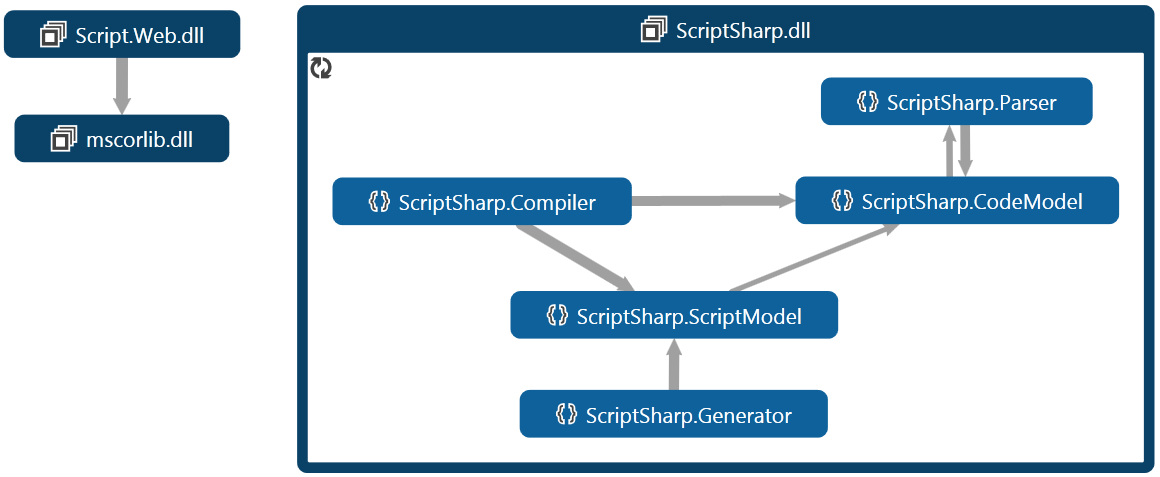
\includegraphics[width=16cm]{resources/images/SimplifiedOverview.png}}
			\end{center}
			\caption{Simplified Script\# architecture overview (dependency diagram).}
			\label{simplifiedOverview}
		\end{figure}


		A thing unique to Script\# is that it defines a modified version of the .NET mscorlib.dll (also shown in figure \ref{simplifiedOverview}) that modifies the .NET core type interfaces to resembles their equivalent JavaScript objects. E.g. the Script\# defined System.String type has a \texttt{CharAt(int index)} function that doesn't exist on the original .NET System.String type but \emph{does} exist on the JavaScript String object. One benefit of the modified mscorlib.dll is that it makes the C\# compiler able to validate the C\# code that represents JavaScript. However, \emph{evaluating} C\# code that uses these modified .NET types will never make sense, as all of the methods and fields on them either returns null, 0, or false, as shown in figure \ref{fig:scriptsharp_net_types}. This implies that the Script\# modified core types can only be used for JavaScript generation.

		\begin{figure}
		\label{fig:scriptsharp_net_types}
			\begin{lstlisting}[language=CSharp,classoffset=1,morekeywords={String}]
namespace System {

  /// <summary>
  /// Equivalent to the String type in Javascript.
  /// </summary>
  [ScriptIgnoreNamespace]
  [ScriptImport]
  public sealed class String {

    ...

    /// <summary>
    /// The number of characters in the string.
    /// </summary>
    [ScriptField]
    public int Length {
      get {
        return 0;
      }
    }

    ...

    /// <summary>
    /// Encodes a single part or component of a URI.
    /// </summary>
    /// <returns>The encoded string.</returns>
    [ScriptAlias("encodeURIComponent")]
    public string EncodeUriComponent() {
      return null;
    }

    ...
  }
}

			\end{lstlisting}
			\caption{Properties and methods on Script\#'s String type}
		\end{figure}

		In short the modified mscorlib.dll file is referenced in one's Visual Studio project (instead of the original one) when a new Script\# project is created. When a Script\# project is compiled a JavaScript file will be generated. This JavaScript file can then be used in other projects (E.g. a Web Forms web application). The C\# source code will not be evaluated.
	% subsection subsection_name (end)


	% \subsection{Microsoft Roslyn} % (fold)
	% \label{ssub:microsoft_roslyn}

	% % subsection microsoft_roslyn (end)

	\subsection{Code Quotations} % (fold)
	\label{ssub:code_quotations}
		Code Quotations is a built-in feature in the F\# language which lets a developer generate an abstract syntax tree that represents the corresponding F\# code. Code Quotations cover the entire F\# language, meaning that theoretically all F\# constructs can be mapped to a corresponding JavaScript construct.

	% subsection code_quotations (end)

	\subsection{Expression Trees} % (fold)
	\label{ssub:expression_trees}
			Expression Trees is a built-in feature in the C\# (and Visual Basic) language that “represents code in a tree-like data structure, where each node is an expression, for example, a method call or a binary operation” (REF MSDN). Expression Trees are often used with LINQ to build dynamic queries, which can be useful when fetching data from a database with filters specified by the user (these filters may be provided through a user interface). Expression Trees can be generated from lambda expressions, and thus it is possible to retrieve a representation of simple pieces of code, such as the following:

			\begin{lstlisting}[language=CSharp,classoffset=1,morekeywords={Func}]
				Func<int, int, bool> function = (a, b) => a > b
			\end{lstlisting}

			or more sophisticated ones such as LINQ queries. 
	% subsection expression_trees (end)

	\subsection{Internal DSL} % (fold)
	\label{ssub:internal_dsl}
		There are different approaches to writing a Domain Specific Languages (DSL) with Internal DSLs you work in your regular language and is therefore also constraint by this language and its features \cite{domain_specific_languages}. Another term for Internal DSL is fluent interface who's central pattern is that of method chaining which is the pattern we somewhat investigated for the use of safe JavaScript representation. In our case we aimed for a Internal DSL that would somewhat the C-like syntax of JavaScript.
	% subsection internal_dsl (end)

\section{Stages When Going From .NET Language to JavaScript} % (fold)
\label{sec:stages_when_going_from_net_language_to_javascript}
	Before discussing different approaches it makes sense to clarify the possible stages in the process of going from a .NET language to JavaScript. The process (displayed in figure \ref{stages}) moves from left to right. Different approaches use different stages.

				\begin{figure}[H]
			\begin{center}
				\centerline{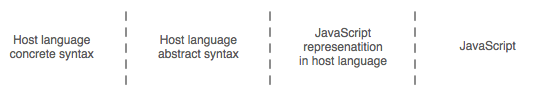
\includegraphics[width=14cm]{resources/images/stages.png}}
			\end{center}
			\caption{Possible approach stages}
			\label{stages}
		\end{figure}

	 From concrete syntax a C\# or F\# abstract syntax tree (AST) can be generated. This AST can be traversed in order to map it to a JavaScript AST. Finally, JavaScript can be generated from the JavaScript AST.
% section stages_when_going_from_net_language_to_javascript (end)

\section{TODO: Possible Approaches} % (fold)
\label{sec:possible_approaches}
	todo text

	\begin{figure}[H]
		\begin{center}
			\centerline{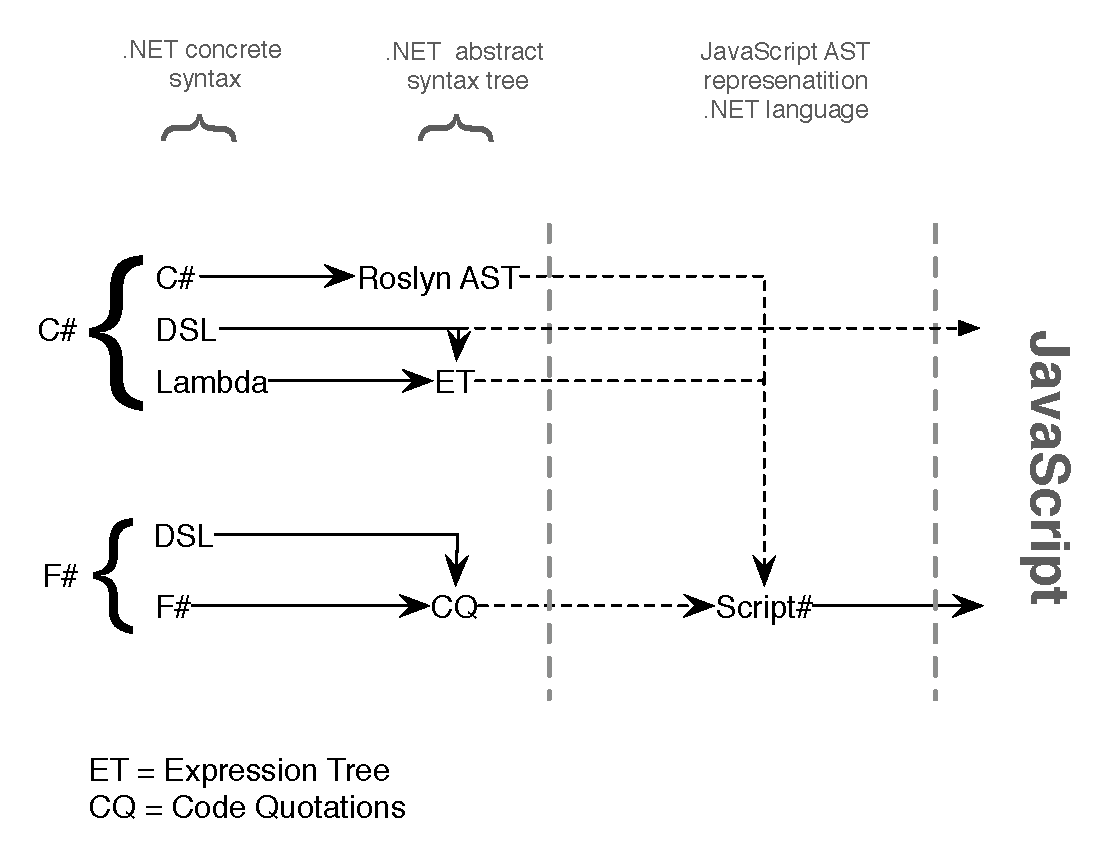
\includegraphics[width=14cm]{resources/images/approachComparison.eps}}
		\end{center}
		\caption{Map of possible approaches. A solid line means that the transition from A to B is given and requires no work on our side. A dashed line means that the transition has to be implemented.}
		\label{approachMap}
	\end{figure}


	\subsection{C\# Approaches} % (fold)
	\label{sub:csharp_approaches}
		
		\subsubsection{C\# to Roslyn to Script\# to JavaScript} % (fold)
		\label{ssub:c_to_roslyn_to_script_to_javascript}
			By using a combination of Roslyn and Script\# it would be possible to generate an AST representing the developers C\# code. The work on our hand in this solution is to map the generated C\# AST to a corresponding Script\# AST representing JavaScript. Script\# would then be able to generate JavaScript from this AST.
		% subsubsection c_to_roslyn_to_script_to_javascript (end)

		\subsubsection{C\# Internal DSL to JavaScript} % (fold)
		\label{ssub:c_internal_dsl_to_javascript}
			To approach the project initially we did some experiments with a C\# internal DSL from which JavaScript was created directly (i.e. the C\# or F\# abstract syntax tree and JavaScript AST stages are skipped). Using helper factory methods, operator overloading and a mechanism to handle block scope we arrived at a DSL syntax that could only be somewhat compared to JavaScript concrete syntax. Furthermore the syntax was a bit verbose which decreased readability. 

			Another problem with the C\# DSL implementation was that the assignment operator C\# could not be overloaded which resulted in inconsistent ways of assigning values to variables. This was a critical problem because wrong use of the ‘\texttt{=}’ operator could cause very subtle errors.

		% subsubsection c_internal_dsl_to_javascript (end)

		\subsubsection{C\# Internal DSL to Expression Trees to JavaScript} % (fold)
		\label{ssub:c_internal_dsl_to_expression_trees_to_javascript}

			We considered a variation of the C\# DSL approach which included the use of Expression Trees (TODO: REF). This DSL would build an AST consisting of Expression Trees from which JavaScript could be generated (i.e. the C\# or F\# abstract syntax tree stage would be included). This approach would somewhat accommodate Server-Client Portability (TODO:REF) because Expression Trees can be dynamically compiled and executed as server side code. However this approach inherits the same problems as the C\# DSL approach.
		% subsubsection c#_internal_dsl_to_expression_trees_to_javascript (end)

		\subsubsection{C\# Lambda to Expression Trees to Script\# to JavaScript} % (fold)
		\label{ssub:c_lambda_to_expression_trees_to_script_to_javascript}
			Instead of building Expression Trees manually as in the previous DSL approach this approach utilizes the possibility to generate Expression Trees from lambda expressions. Using lambda expressions would imply that C\# concrete syntax could be used and not a DSL. Therefore the DSL related problems discussed above would be avoided which makes this approach superior to the DSL approaches. However an Expression Tree cannot be generated from lambda \emph{statements} this implies that the use of statements would not be possible with this approach. The use of statements is somewhat important when trying to represent JavaScript so this was a critical shortcoming for this approach.
		% subsubsection c_lambda_to_expression_trees_to_script#_to_javascript (end)

	% subsection csharp_approaches (end)

	\subsection{F\# Approaches} % (fold)
	\label{sub:f_approaches}
	
		\subsubsection{F\# Internal DSL to Script\# to JavaScript} % (fold)
		\label{ssub:f_internal_dsl_to_script_to_javascript}
			An alternative to an C\# internal DSL is an F\# internal DSL. The problem with not being able to overload the assignment operator would not be an issue in F\#. It is even possible to implement new operators consisting of one or more characters from a given set, consequently making it possible to implement some special JavaScript operators such as strict equal (===).
		% subsubsection f_internal_dsl_to_script_to_javascript (end)

		\subsubsection{F\# Code Quotations to Script\# to JavaScript} % (fold)
		\label{ssub:f_code_quotations_to_script_to_javascript}
			An alternative to using C\# and Roslyn is F\# and Code Quotations. As with Roslyn, the work on our hand would be to map the F\# AST to it's corresponding Script\# JavaScript AST. A disadvantage of using Code Quotations is that they require the developer to know a different language from the one in which ASP.NET Web Forms applications are typically written (C\#). This would probably not be a very great barrier if the syntax of the language didn't vary as much as F\# does from C\#. Also, C\# and JavaScript are somewhat similar in syntax, whereas F\#'s and JavaScripts syntaxes are beyond comparison. A problem related to F\#'s syntax is that the mapping between the F\# AST and the Script\# JavaScript AST could possibly be more difficult than with C\# and Roslyn and thus impose a greater work load on us.
		% subsubsection f_code_quotations_to_script_to_javascript (end)

	% subsection f_approaches (end)



	% \subsection{Internal DSL Approaches} % (fold)
	% \label{ssub:internal_dsl_approaches}

	% 	The Internal DSL approaches have been separated into two categories. The first where the DSL is used to build a host language AST which later can be mapped to a target language AST. The second where the target language AST is created directly (i.e.\ the Host Language Abstract Syntax stage is skipped). One significant difference in these two approaches has to do with the possibility of executing code both on server side and client side. When generating the host language AST before mapping to the target language AST its easier to also execute the code in the host language context through dynamic compilation of the host language AST (this approach is discussed in xx TODO).
	
	% 	\subsubsection{Internal DSL Directly to JavaScript AST} % (fold)
	% 	\label{sub:internal_dsl_directly_to_javascript_ast}
		
	% 		When utilizing an internal DSL one would need classes for representing primitive types, expression, statements etc. All the target language features that one will make available needs to be mapped to a DSL representation. Every DSL call would then instantiate an equivalent target language AST node.

	% 		One thing important to consider when creating a DSL representing a different language is its syntax. The DSL syntax should resemble the target language concrete syntax so that the DSL is easily utilized by the target users. At the same time, it should make the verbose instantiation (see example below) of host abstract syntax less cumbersome.

	% 		todo: redo code example

	% 	% subsection internal_dsl_directly_to_javascript_ast (end)

	% 	\subsubsection{C\# DSL} % (fold)
	% 	\label{sub:cs_dsl}

	% 		To approach the project initially we did some experiments with a DSL (in C\#) that created a JavaScript AST directly (i.e. the .NET Abstract Syntax tree stage was skipped) (TODO: See appendix for class diagram and maybe description of scope / block handling mechanism etc.). Using helper factory methods (to create AST nodes), operator overloading and a scope and block handling mechanism (utilizing Statement Lambdas) one can arrive at a DSL syntax that could be somewhat compared to concrete syntax (see example below).

	% 		todo: redo code example

	% 		However, there are different problems with this approach. First of all the syntax doesn't exactly resemble regular C\# or JavaScript. This implies that there will be a learning effort before the DSL can be used. Furthermore the syntax is a bit verbose and readability is also decreased a bit.

	% 		Another problem with the C\# DSL implementation is that the initial declaration and assignment of the variable ``i'' is done using ``='' operator where any subsequent assignments should be done using the ``Assign(...)'' method (or possibly through overloading an existing operator e.g. \texttt{\%=}). The main reason for this is that it is not possible to override the assignment operator in C\# (QUOTATION). This is a critical problem because if the regular C\# assignment operator, \texttt{=}, was used incorrectly by mistake it would not trigger any exceptions and therefore cause a difficult to debug error.  The example below shows exactly this. The variable ``i'' is assigned in an incorrect manner after its initial declaration according to the DSL syntax.

	% 		todo: redo code example
		
	% 	% subsection subsection_name (end)

	% 	\subsubsection{F\# DSL} % (fold)
	% 	\label{sub:fs_dsl}
	% 		The problem with not being able to overload the assignment operator (illustrated in figure todo: REF) would not be an issue in F\# as the assignment operator could be overloaded. Furthermore it is even possible to implement new operators consisting of one or more characters from a given set of characters, consequently making it possible to implement some special JavaScript operators such as strict equal (===).

	% 		One problem though with the F\# DSL approach is the fact that the F\# native syntax and programming paradigm (e.g. the use of immutable types) is radically different from that of JavaScript (and C\# for that matter). This would imply a steep learning curve according to our target user as one would have to learn the F\# syntax and programming paradigm together with the DSL. Even if F\# was the language of choice there would be other powerful language features (i.e.\ Code Quotations) that might bias one toward a different approach (see section \ref{sub:using_fs_code_quotations}).
	% 	% subsection fs_dsl (end)

	% 	\subsubsection{DSL to .NET AST} % (fold)
	% 	\label{sub:dsl_to_net_ast}
	% 		To accommodate server client portability one option in C\# is to utilize Expression Trees. With this approach the DSL would build a .NET AST represented as an Expression Tree which hereafter could be mapped to JavaScript. The .NET AST can also be compiled into host language executable code using the Compile() feature (todo: QUOTATION) on Expression Trees. With an F\# DSL approach a similar pattern could be achieved with Code Quotations (the Expr type). A more straightforward solution to the mixed side execution goal would though be to not use a DSL. Instead one would use the concrete syntax of host language. Then utilize dynamic compilation to retrieve the host language AST which is what we'll discuss in the next section (todo: REF ``Using Roslyn'').
	% 	% subsection dsl_to_host_ast (end)
	% % subsubsection internal_dsl_approaches (end)


	% \subsection{Host Language Approaches} % (fold)
	% \label{sub:host_language_approaches}
	% 	Instead of using an internal DSL, tools (or in some cases language features) exist to generate AST’s from native host language code. These can be traversed and processed as desired by the programmer.

	% 	As tools handle the generation of a host language AST, the workload imposed on the programmer by using this approach is considerably smaller than using e.g. an internal DSL. When using an internal DSL it is up to the programmer to implement a library that represents its concrete syntax.

	% 	The workload is also lightened on the developer. When using tools to generate a host language AST it is possible for the developer to write native code and have it converted to JavaScript instead of having to learn how to use a new library.

	% 	As the host language AST is generated from native host language code it is possible to use the same code on both client side and server side, as the client side code is generated from the server side code. This is very useful with cases such as form validation as it is not necessary for the developer to write the same logic in two different languages. Furthermore, it allows the developer to generate client side code reusing code from previous C\# projects.

	% 	Another benefit of using native host language code, is the possibility of testing on server side. As the code is able to run and evaluate on server side, the developer won't have to write tests in two different languages as the unit testing framework has effectively also been applied to the client side code.

	% 	One disadvantage of using an AST generated from a native host language is that there are no restrictions on what the developer might do. The scope of the project is set by our case study, and as such, our solution will be unable to convert every single construct of an entire language. Should the developer choose to use a language construct that our solution does not support, it will result in a (server-side) runtime error, whereas a DSL would already discover this on compile time. The reason for this is the intrinsic limiting nature of a DSL (todo: REF BOOK: Domain Specific Languages + clarify intrinsic limited nature).

	% 	\subsection{Using F\# Code Quotations} % (fold)
	% 	\label{sub:using_fs_code_quotations}
	% 		The main disadvantage of using Code Quotations is that they require the end user to know a different language from the one in which ASP.NET WebForms Applications are typically written (C\#). This would probably not be a very great barrier if the syntax of the language didn't vary as much as F\# does from C\#. Also, C\# and JavaScript are somewhat similar in syntax, whereas F\#'s and JavaScripts syntaxes are beyond comparison.
	% 	% subsection using_f#_code_quotations (end)

	% 	\subsection{Using C\# Expression Trees} % (fold)
	% 	\label{sub:using_cs_expression_trees}
	% 		A major pitfall using Expression Trees is that they cannot be generated from lambda statements, which prevents the possibility of generating AST’s from blocks of code.
	% 	% subsection using_C\#_expression_trees (end)

	% 	\subsection{Using Roslyn} % (fold)
	% 	\label{sub:using_roslyn}
	% 		Roslyn combines the advantages of Code Quotations and Expression Trees by allowing the generation of an AST from every C\# construct (including blocks), and avoiding the unfamiliar F\# syntax.
		% subsection using_roslyn (end)
	% subsection host_language_approaches (end)

% section possible_approaches (end)

\section{Deciding on Approach} % (fold)
\label{sec:deciding_on_approach}
	In the previos sections we have described varios technologies, how they can be used in combination to form approaches, and some of the benefits and disadvantages of these approaches. To make a final decission on which approach to choose for implementation, an approach matrix has been made. The matrix evaluates the different approaches based on 9 different critera. The approach matrix is shown in figure \ref{approachMatrix}, and below each criterion is explained. All approaches accommodate JavaScript-HTML consistency which is why no ratings are given on this matter.

	\begin{figure}
		\begin{center}
			\centerline{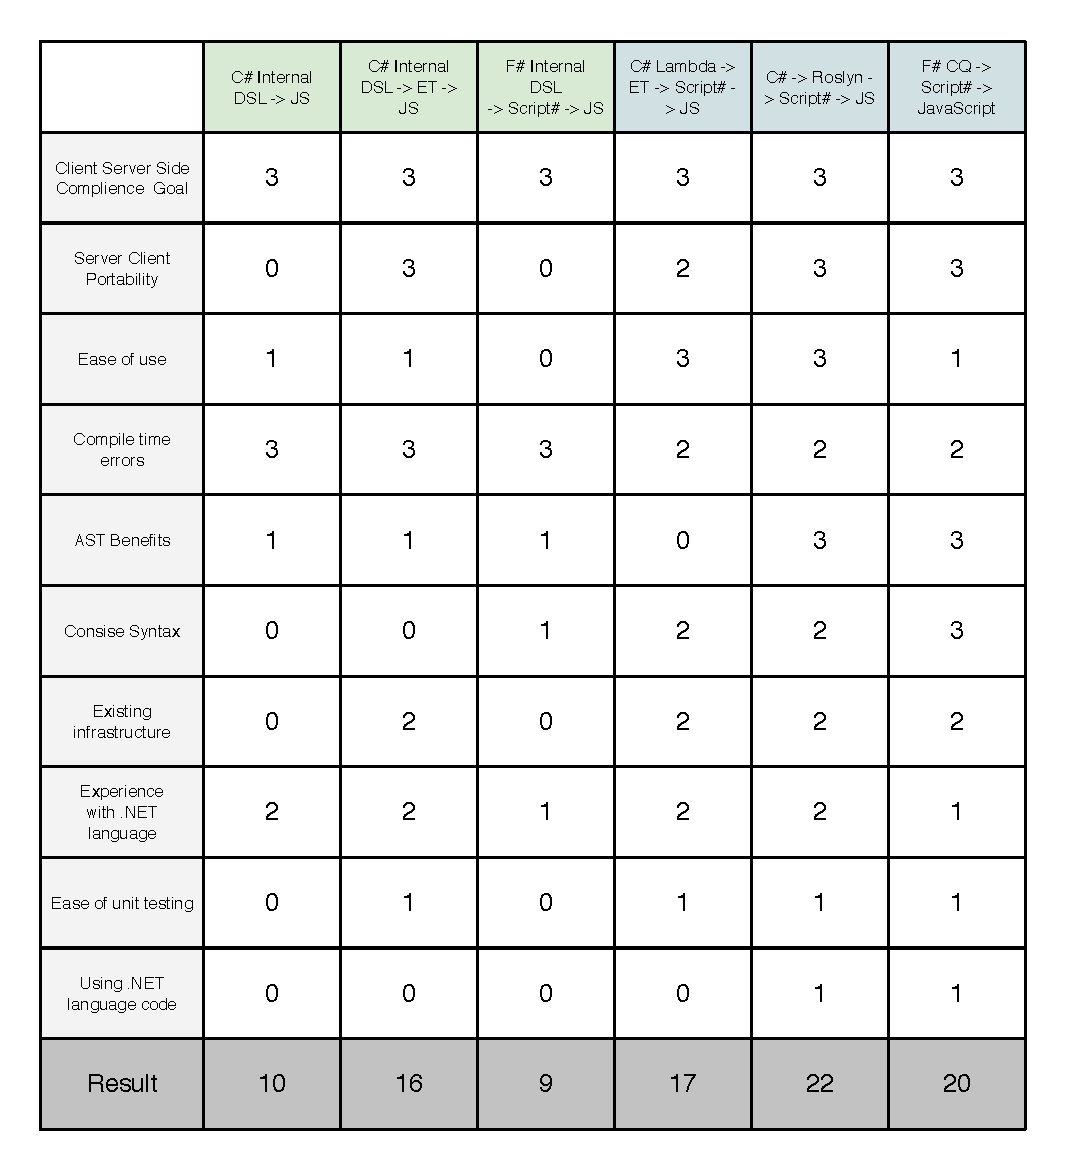
\includegraphics[width=16cm]{resources/images/approachmatrix.eps}}
		\end{center}
		\caption{Approach Matrix.}
		\label{approachMatrix}
	\end{figure}

	\begin{itemize}
		\item \textbf{Server Client Portability} The ability to generate JavaScript from working server side code
		\item \textbf{Ease of Use} How easy the approach is to use for the developer
		\item \textbf{Compile Time Errors} Amount of errors this approach will catch on compile time
		\item \textbf{AST Benefits} How easily the developer's code can be converted to an AST
		\item \textbf{Consise Syntax} How concise the syntax of the approach will be
		\item \textbf{Existing Infrastructure} The degree to which the approach makes use of existing C\# or F\# constructs
		\item \textbf{Experience with .NET Language} How well we know the language in which the approach is implemented
		\item \textbf{Ease of Unit Testing} How easily the developer can unit test his code with the approach
	\end{itemize}

	We have rated approach criteria from 0 to 3 where three is the best. With the approach matrix as support we decided to implement the C\# to Roslyn to Script\# to JavaScript approach. The approach was named Mixed Side C Sharp (MiCS).

	\FloatBarrier

	\subsection{MiCS: Mixed Side C\#} % (fold)
	\label{sub:mics_mixed_side_csharp}
	MiCS will use Roslyn and Script\# in combination. Roslyn will be used to generate an AST representing the developer's C\# source code. The core functionality of MiCS will be to map this generated AST to a Script\# JavaScript AST. Script\#'s JavaScript generator will be used to generate the actual JavaScript source code. In the following chapters the design and implementation of this approach will be described in detail.

	% subsection mics_mixed_side_csharp (end)

% section deciding_on_approach (end)